\documentclass[a4paper, 10pt]{article}
\usepackage[margin=0.5in]{geometry}

\usepackage{blindtext}
\usepackage{multicol}
\usepackage{booktabs}
\usepackage{amsmath}
\usepackage{mathtools}
\usepackage{float}
\usepackage{graphicx}
\usepackage{enumitem}

\graphicspath{ {../outputs/}{../data/} }


\setlength{\columnsep}{1cm}
\title{ENPM 673: Perception for Autonomous Robots - Project 1}
\author{Aswath Muthuselvam}
\date{26th Feb 2022}

\begin{document}
\maketitle
\newlist{contract}{enumerate}{10}
\setlist[contract]{label*=\arabic*.}
\setlistdepth{10} 

\begin{multicols}{2}
	
\section{Problem 1}
\subsection{A) AR Code detection}

A robot need to make sense of it's surroundings and able to localize itself with respect to it's surrounding environment. Problem 1a involves detection of AR Code. An AR Code is a marker that is used as an easy method of perceiving the environment by using simple algorithms rather than having to understand the entirety of the scene.

The detection of this tag involves multiple steps:
\begin{enumerate}
	\item Pass the image through High Pass filter
	\begin{contract}
		\item Take Fourier Transform
		\item Frequency shift 
		\item Prepare a mask
		\item Apply the mask to filter the low frequency components.
	\end{contract}
		\item Apply inverse Fourier transform.
		\item Apply FFTShift
	
\end{enumerate}

\begin{figure}[H]
	\centering
	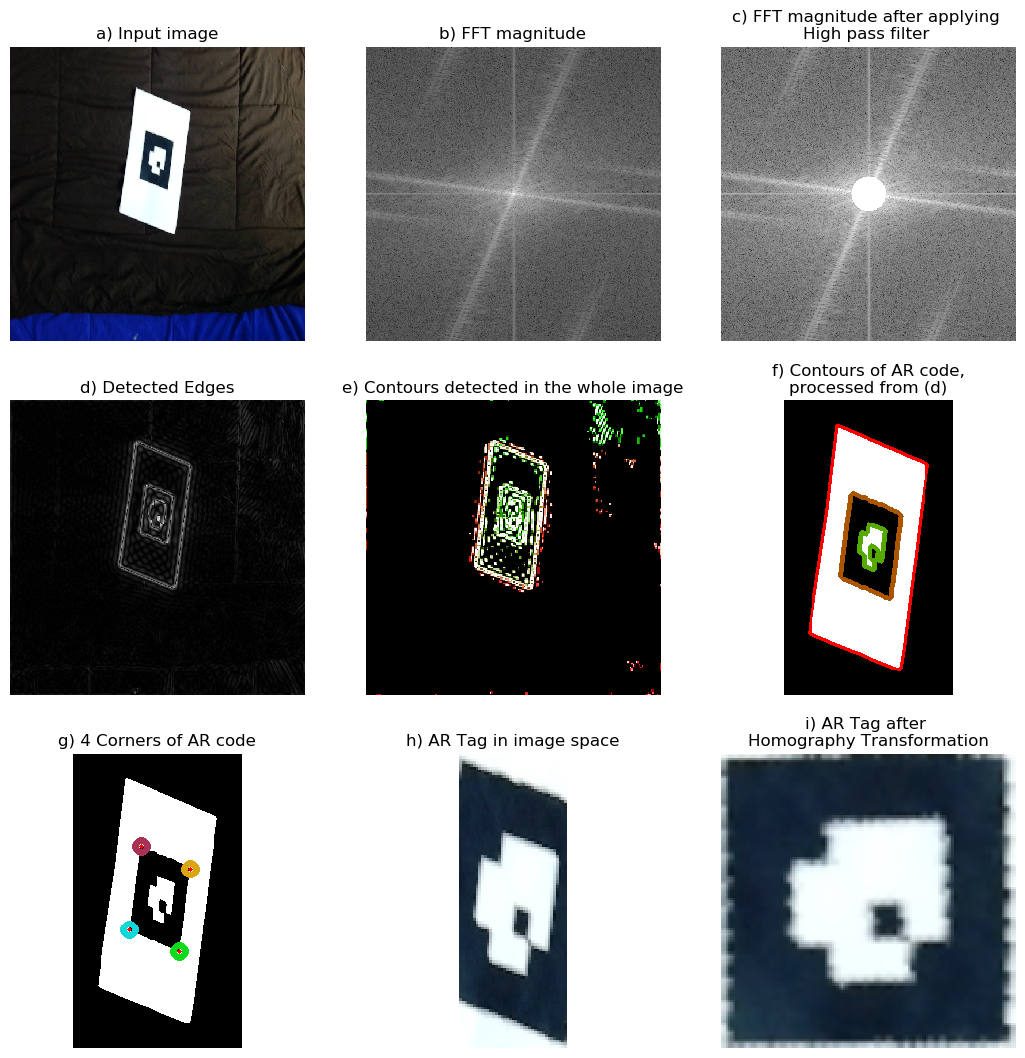
\includegraphics[width=\columnwidth]{/Q1/ARDetectionUsingFFt.png}
	\caption{AR Tag localization with FFT and Homography}
	\label{fig:FFT}
\end{figure}

\blindtext

The homography transformation matrix is given by:
\[
\begin{bmatrix}
x^{'} \\
y^{'} \\
w
\end{bmatrix} =
H\begin{bmatrix}
x \\
y \\
1
\end{bmatrix} = 
\begin{bmatrix}
h_{11} & h_{12} & h_{13}\\
h_{21} & h_{22} & h_{23}\\
h_{31} & h_{32} & h_{33}
\end{bmatrix}
\begin{bmatrix}
x \\
y \\
1
\end{bmatrix}
\]

\subsection{B) AR Code Decoding}
An AR Code has two orthogonal protrusions on one corner. Using this feature, the orientation of the AR Code can be determined. The AR Code decoded by splitting the image into a 8x8 Grid and summing the pixel intensities in each grid.
\begin{figure}[H]
	\centering
	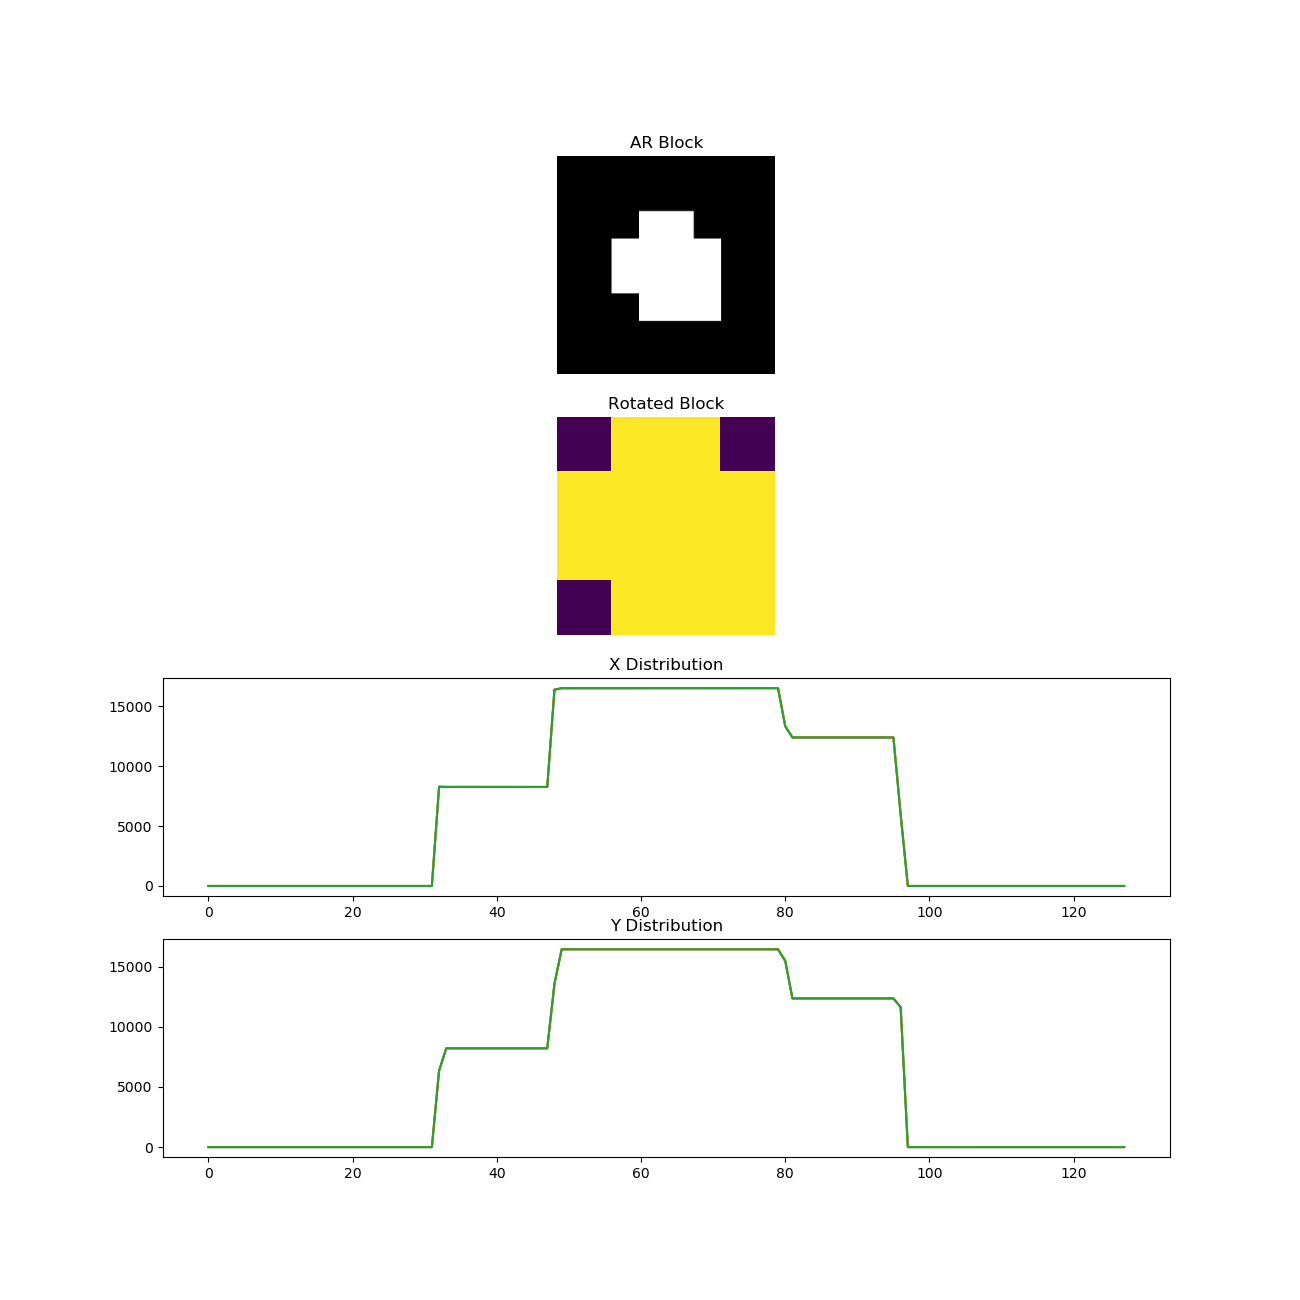
\includegraphics[width=\columnwidth]{/Q1/AR_Code_Decode.png}
	\caption{Decoding the AR Code}
	\label{fig:ARDecode}
\end{figure}


\section{Problem 2}


\section{Extra Credit}

Two types of Edge detection are performed on the Cityscape image show in Figure: \ref{fig:cityscape}. The first method is by using Canny edge detection and the second is by using DexiNed. DexiNed(Dense EXtreme Inception Network for Edge Detection) is a CNN based Edge detector.
\begin{figure}[H]
	\centering
	\includegraphics[width=\columnwidth]{/cityscape1.png}
	\caption{Canny Edge detection}
	\label{fig:cityscape}
\end{figure}


\begin{figure}[H]
	\centering
	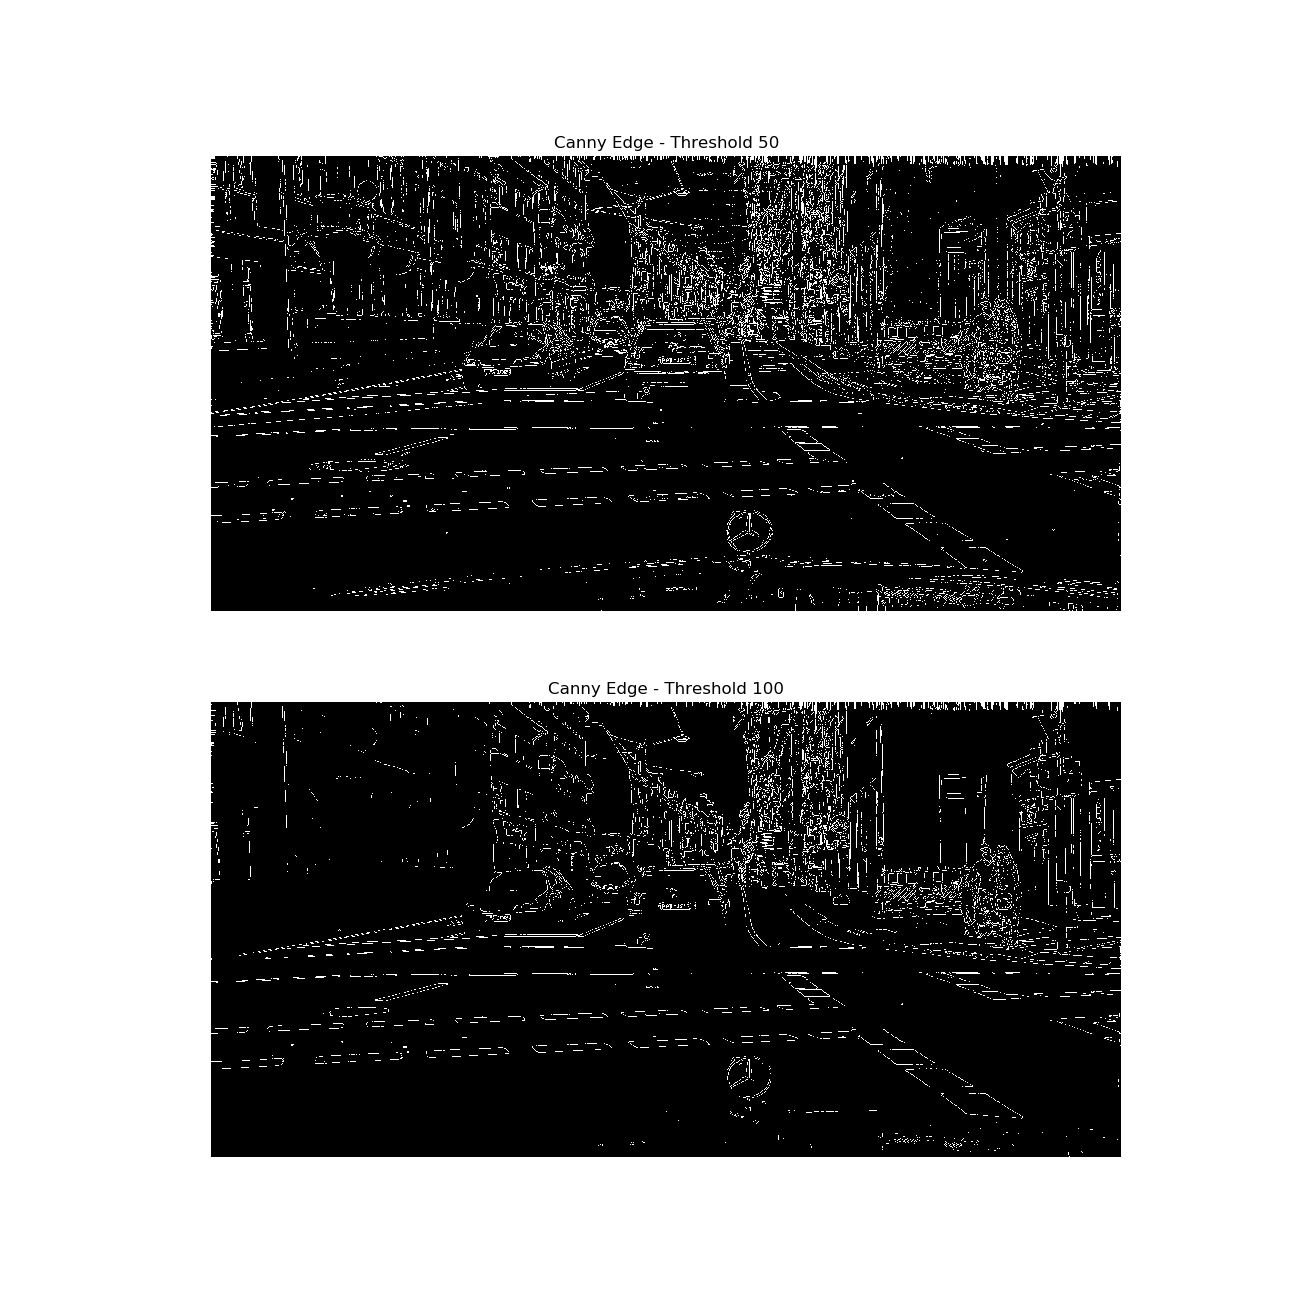
\includegraphics[width=\columnwidth]{/ExtraCredit/CannyEdge.png}
	\caption{Canny Edge detection}
	\label{fig:Canny}
\end{figure}

\begin{figure}[H]
	\centering
	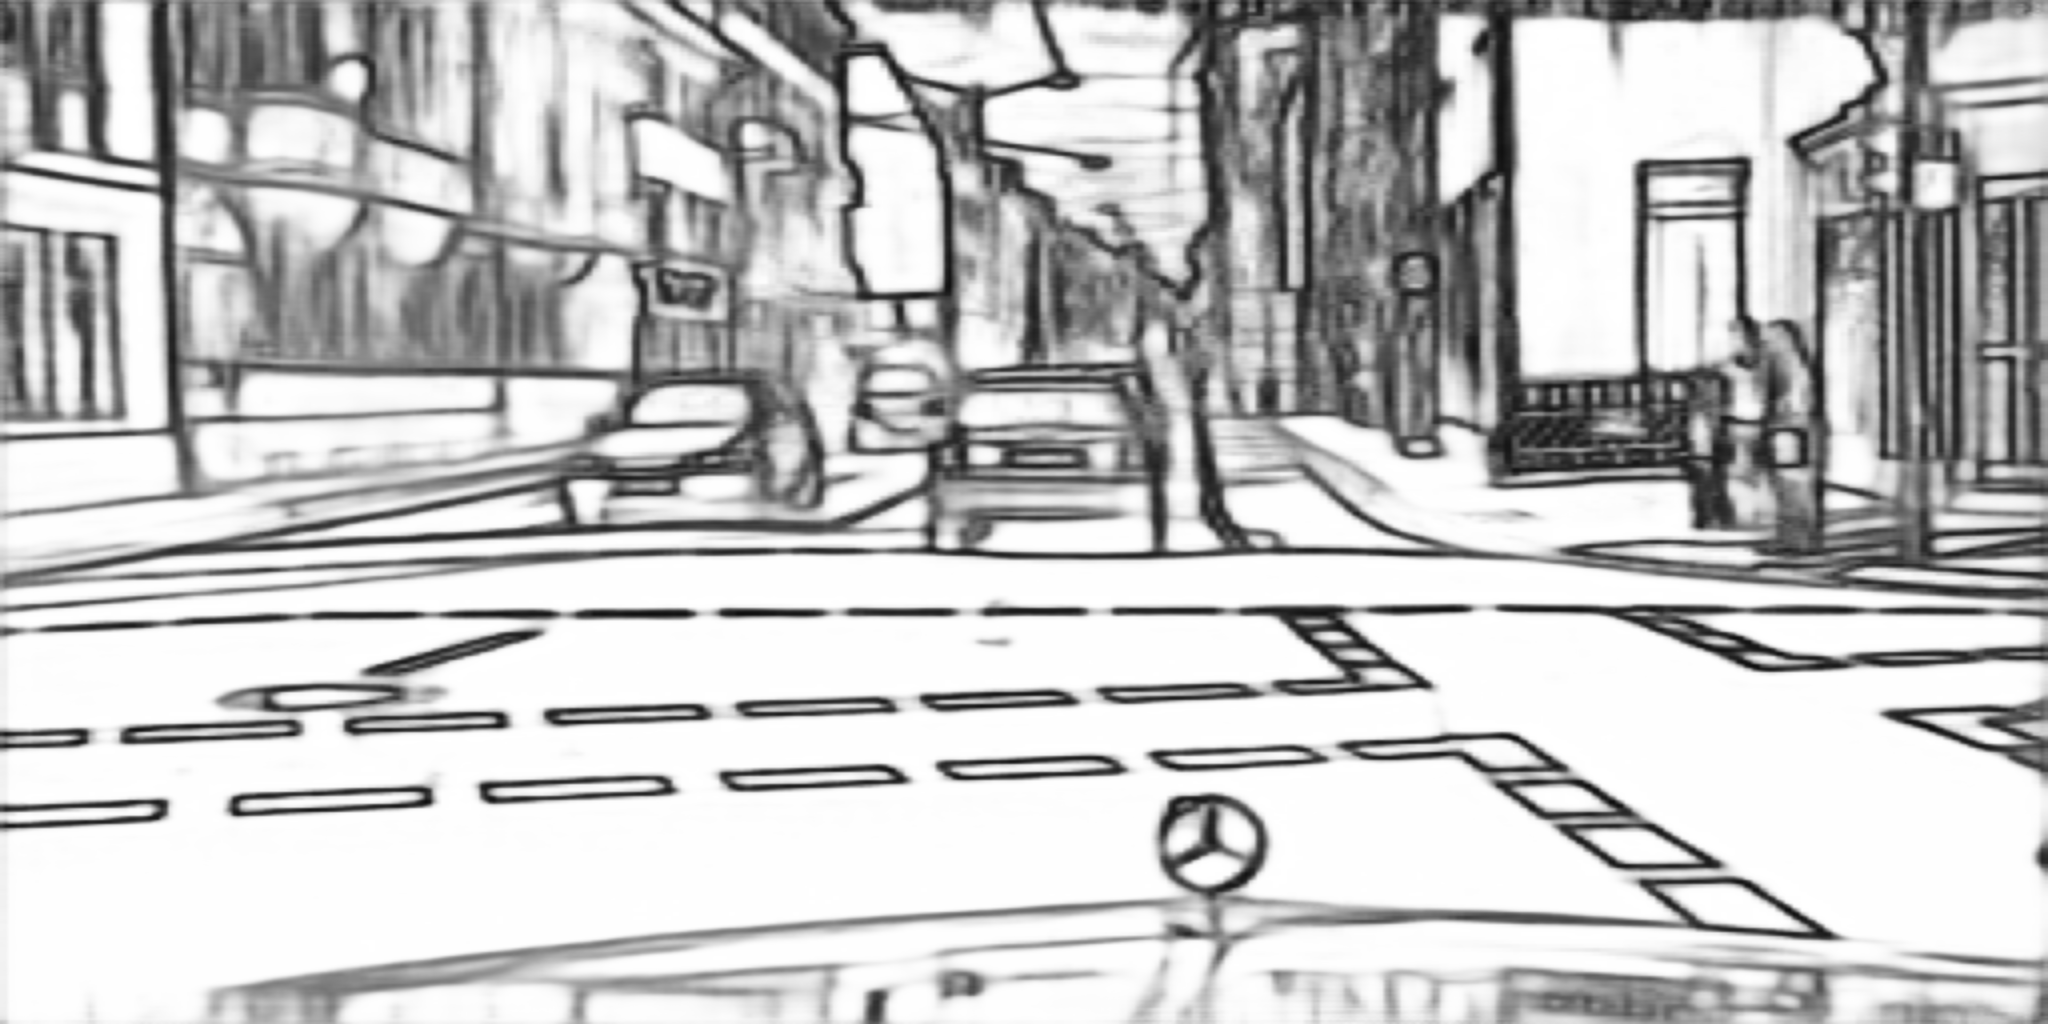
\includegraphics[width=\columnwidth]{/ExtraCredit/cityscape_avg.png}
	\caption{Edge Detection with DexiNed}
	\label{fig:DexiNed}
\end{figure}
	
	
\end{multicols}
	
\end{document}
